\documentclass[a4paper, 12pt]{article}
\usepackage{graphicx}
\usepackage[margin=2cm]{geometry}
\usepackage[hidelinks]{hyperref}
\usepackage[croatian]{babel}
\usepackage[sorting=none]{biblatex}
    \addbibresource{ref.bib}
\usepackage{float}

% Boje za kod:
\usepackage{xcolor,graphicx}
\usepackage{listings}

\definecolor{solarized-base03}{RGB}{0, 43, 54}
\definecolor{solarized-base02}{RGB}{7, 54, 66}
\definecolor{solarized-base01}{RGB}{88, 110, 117}
\definecolor{solarized-base00}{RGB}{101, 123, 131}
\definecolor{solarized-base0}{RGB}{131, 148, 150}
\definecolor{solarized-base1}{RGB}{147, 161, 161}
\definecolor{solarized-base2}{RGB}{238, 232, 213}
\definecolor{solarized-base3}{RGB}{253, 246, 227}
\definecolor{solarized-yellow}{RGB}{181, 137, 0}
\definecolor{solarized-orange}{RGB}{203, 75, 22}
\definecolor{solarized-red}{RGB}{220, 50, 47}
\definecolor{solarized-magenta}{RGB}{211, 54, 130}
\definecolor{solarized-violet}{RGB}{108, 113, 196}
\definecolor{solarized-blue}{RGB}{38, 139, 210}
\definecolor{solarized-cyan}{RGB}{42, 161, 198}
\definecolor{solarized-green}{RGB}{133, 153, 0}

\lstset{
  basicstyle=\footnotesize\ttfamily\color{solarized-base00},
  keywordstyle=\color{solarized-blue}\bfseries,
  commentstyle=\color{solarized-base1},
  stringstyle=\color{solarized-cyan},
  identifierstyle=\color{solarized-violet},
  numberstyle=\tiny\color{solarized-base01},
  numbers=left,
  firstnumber=1,
  stepnumber=1,
  showstringspaces=false,
  tabsize=4,
  frame=none,
  framerule=1pt,
  framexleftmargin=5pt,
  framexrightmargin=5pt,
  framextopmargin=3pt,
  framexbottommargin=3pt,
  backgroundcolor=\color{solarized-base3},
  rulecolor=\color{solarized-base01},
  breaklines=true,
  breakatwhitespace=true,
  language=C++
}


\begin{document}
\noindent
Univerzitet u Sarajevu\\
Elektrotehnički fakultet\\
Predmet: Uvod u digitalnu obradu slike\\
Predmetni profesor: prof. dr Emir Sokić\\
Autor: Berina Biberović\\
Akademska godina: 2022/2023.


\begin{center}
    \section*{Tutorijal 4}
    \subsection*{Detekcija ivica na slici}
\end{center}

\subsection*{Sobel operator}

Sobel operator je operator diskretnog diferenciranja koji računa aproksimaciju gradijenta od funkcije intenziteta slike. Sobel operator kombinira Gaussovo izglađivanje i diferenciranje.

U sljedećem primjeru će biti pokazano kako iskoristiti Sobel operator da se dobiju ivice na slici. OpenCV ima ugrađenu funkciju \lstinline{cv::Sobel} koja primjenjuje operator nad datom slikom, tako da mi ne moramo sami računati matrice i množiti ih koje Sobel operator traži. Ova implementirana funkcija unutar OpenCV-a je svakako optimizirana i dobro napisana.

\begin{lstlisting}
#include <opencv4/opencv2/highgui.hpp>
#include <opencv4/opencv2/core/mat.hpp>
#include <opencv4/opencv2/imgproc.hpp>

int main() {

    // Ucitavanje slike:
    cv::Mat slika = cv::imread("../nonaka_miho.jpg", cv::IMREAD_COLOR);

    // Prebacivanje u grayscale:
    cv::Mat gray;
    cv::cvtColor(slika, gray, cv::COLOR_BGR2GRAY);

    // Dodavanje blura na grayscale sliku:
    cv::Mat blur;
    cv::GaussianBlur(gray, blur, cv::Size(3, 3), 0, 0, cv::BORDER_DEFAULT);

    // Sobel:
    cv::Mat sobel;
    int ddepth = CV_8U;
    cv::Sobel(blur, sobel, ddepth, 0, 1, 3, 1, 0, cv::BORDER_DEFAULT);

    cv::imshow("Originalna", slika);
    cv::imshow("Blur", blur);
    cv::imshow("Nakon Sobela", sobel);

    cv::waitKey();

    return 0;
}
\end{lstlisting}

U gore navedenom kodu je prikazan postupak primjene Sobel transformacije u OpenCV-u. Prvo je potrebno učitanu sliku prebaciti u \textit{grayscale}, nakon toga je potrebno uz pomoć \lstinline{cv::GaussianBlur} funkcije primijeniti \textit{blur} na sliku kako bi se šum odstranio sa slike (u ovom slučaju smo koristili kernel veličine $3 \times 3$. Nakon toga primjenjujemo Sobel funkciju u OpenCV-u kojoj prosljeđujemo \textit{blur}-anu sliku, izlaznu sliku iz Sobela, dubinu izlazne slike, red izvoda po $x$, red izvoda po $y$, veličinu kernela, \textit{scaling} faktor za izračunate vrijednosti izvoda, vrijednost koja se dodaje na rezultate prije nego što se upiše u izlaznu sliku i način ekstrapolacije piksela.

Rezultati su prikazani na slikama \ref{sl_miho} i \ref{sl_sobel_miho}. Vidimo da su uspješno prikazane ivice (obrisi) djevojke bijelom bojom na tamnoj pozadini.

\begin{figure}[H]
    \minipage{0.49\textwidth}
        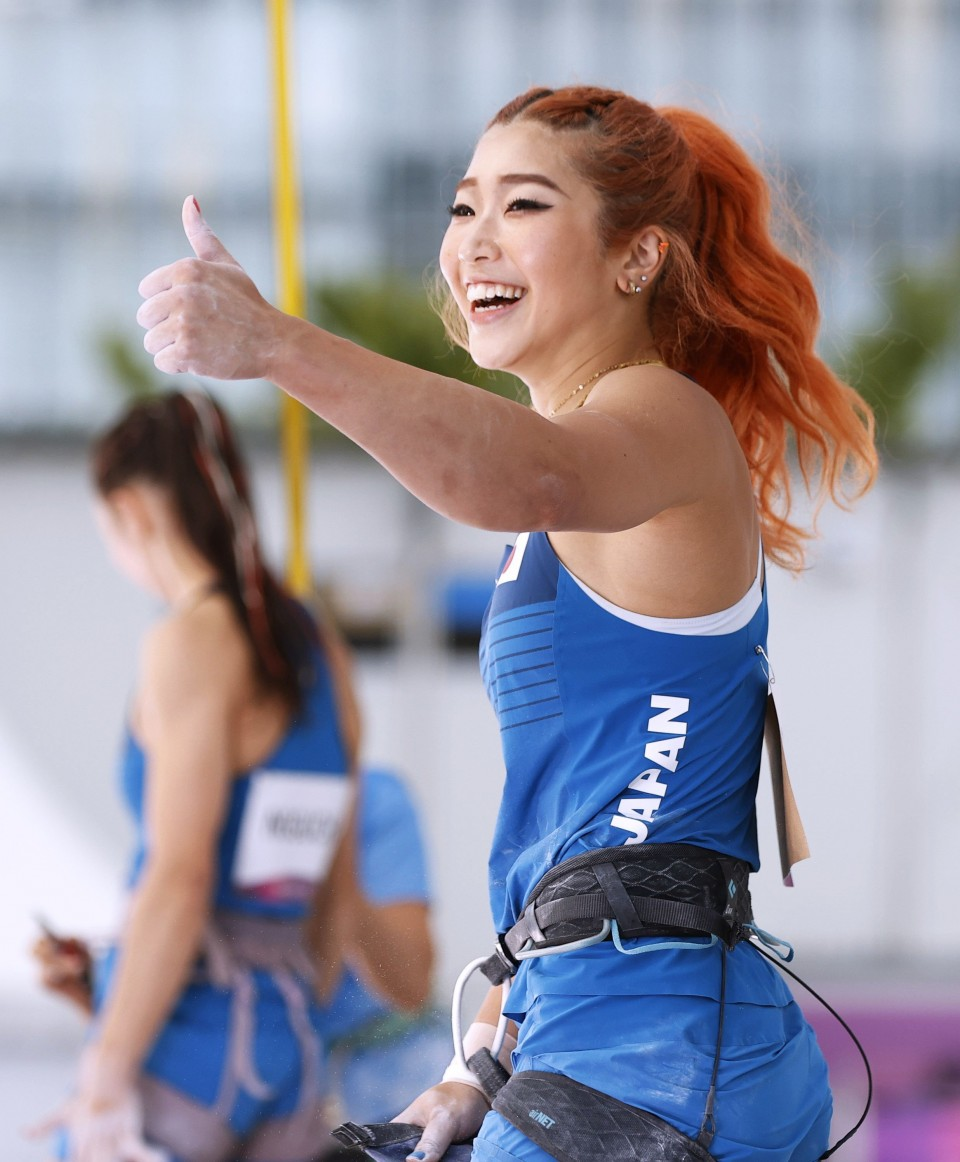
\includegraphics[width=\linewidth]{Slike/nonaka_miho.jpg}
        \caption{Originalna slika\cite{nonaka_miho}}\label{sl_miho}
    \endminipage\hfill
    \minipage{0.49\textwidth}
        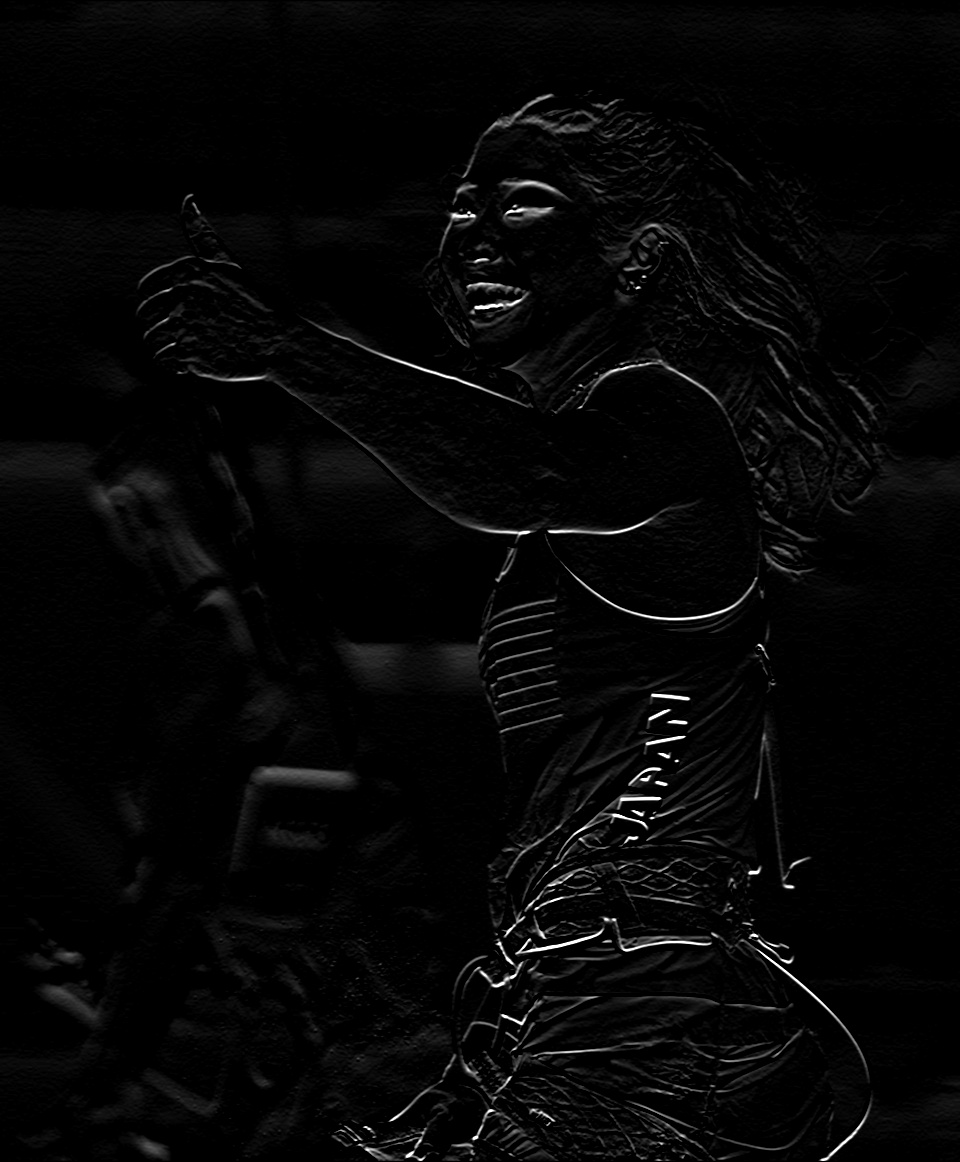
\includegraphics[width=\linewidth]{Slike/sobel.jpg}
        \caption{Slika nakon Sobel transformacije}\label{sl_sobel_miho}
    \endminipage\hfill
\end{figure}

\subsection*{Canny operator}

Canny detektor ivica je popularan algoritam kojeg je napravio John F. Canny. To je algoritam sa više etapa, u koje nećemo ulaziti detaljno u ovom tutorijalu. Ono što je nama važno jeste kako implementirati već gotovi Canny algoritam u OpenCV-u. OpenCV ima gotovu funkciju za Canny operator \lstinline{cv::Canny}.

\begin{lstlisting}
#include <opencv4/opencv2/highgui.hpp>
#include <opencv4/opencv2/core/mat.hpp>
#include <opencv4/opencv2/imgproc.hpp>

int main() {

    // Ucitavanje slike u grayscale-u:
    cv::Mat gray = cv::imread("../nonaka_miho.jpg", cv::IMREAD_GRAYSCALE);

    // Canny transformacija:
    cv::Mat canny;
    int t1, t2, aperture = 3;

    cv::namedWindow("Trackbars");
    cv::createTrackbar("Threshold 1", "Trackbars", nullptr, 255);
    cv::createTrackbar("Threshold 2", "Trackbars", nullptr, 255);

    do {

        // Uzimamo vrijednosti t1 i t2 preko trackbarova:
        t1 = cv::getTrackbarPos("Threshold 1", "Trackbars");
        t2 = cv::getTrackbarPos("Threshold 2", "Trackbars");

        cv::Canny(gray, canny, t1, t2, aperture, false);
        cv::imshow("Canny - aperture = 3", canny);
        cv::imshow("Grayscale slika", gray);

    }while(cv::waitKey() != 'q');

    return 0;
}
\end{lstlisting}

Prethodni isječak koda pokazuje kako se može iskoristiti \lstinline{cv::Canny} funkcija kako bi se ivice slike mogle izdvojiti. Naime, bilo je potrebno ovdje napraviti \textit{trackbar}-ove za treći i četvrti parametar koji prima funkcija, kako bi se što bolje izdvojile ivice. U ovakvom programu korisnik pomjeranjem \textit{trackbar}-ova namiješta parametre za Canny operator. Bitno je naglasiti da je peti parametar koji prima funkcija stavljen fiksno na \lstinline{aperture = 3}. Taj parametar se može mijenjati, ukoliko je to potrebno. 

\subsubsection*{Zadatak 1}

Korištenjem prethodnog koda naći ručno optimalne vrijednosti za parametre \lstinline{t1} i \lstinline{t2}.

\subsubsection*{Zadatak 2 - važan za testove}

Istražiti OpenCV funkciju \lstinline{cv::HoughLines} koja se koristi u laboratorijskoj vježbi broj 4. Nakon što istražite tu funkciju, primijenite je na proizvoljnu sliku koristeći Canny operator koji smo naučili na ovom tutorijalu. Kada dobijete linije kao rezultat funkcije \lstinline{cv::HoughLines}, potrebno je da naučite kako ih iscrtati, što je dato u sljedećem isječku koda:

\begin{lstlisting}
    for(int i = 0; i < linije.size(); i++) {

        double rho = linije[i][0], theta = linije[i][1];

        cv::Point p1, p2;

        double a = std::cos(theta), b = std::sin(theta);
        double x0 = rho * a, y0 = rho * b;

        p1.x = cvRound(x0 + 1000 * (-b));
        p1.y = cvRound(y0 + 1000 * (a));
        p2.x = cvRound(x0 - 1000 * (-b));
        p2.y = cvRound(y0 - 1000 * (a));

        // Iscrtavamo linije na slici crvenom bojom:
        cv::line(slika_na_kojoj_iscrtavamo_linije, p1, p2, cv::Scalar(0, 0, 255), 3, cv::LINE_AA);
   }
\end{lstlisting}

\subsection*{Napomene}

Korištena tema za prikaz C++ koda na tutorijalima je \href{https://ethanschoonover.com/solarized/}{\lstinline{solarized}}\cite{solarized}.

\printbibliography


\end{document}
